\documentclass[a4paper, 10pt, conference]{ieeeconf}


%%%%%%%%%%%%
% Packages %
%%%%%%%%%%%%

\usepackage[utf8]{inputenc}
\usepackage[T1]{fontenc}

\usepackage{amsmath}
\usepackage{amssymb}

\usepackage{graphicx}
\usepackage{hyperref}
\usepackage{tabularx}

\usepackage{cite}

\usepackage{layout}
\usepackage{lipsum}

\usepackage{gensymb}


%%%%%%%%%%%%
% Settings %
%%%%%%%%%%%%

\makeatletter
\def\title#1{\gdef\@title{\LARGE\bfseries#1}}
\makeatother
\setlength{\topmargin}{0pt}
\setlength{\oddsidemargin}{-18pt}


%%%%%%%%%%
% Header %
%%%%%%%%%%

\title{INFO0948-1 : Midterm report}
\author{Maxime \textsc{Meurisse} (s161278) \and Valentin \textsc{Vermeylen} (s162864)}


%%%%%%%%%%%%
% Document %
%%%%%%%%%%%%

\begin{document}
    % ----- Header ----- %
    
    \maketitle
    \thispagestyle{plain}
    \pagestyle{plain}
    
    
    % ----- Content ----- %
    
    \section{Short commented video and code}
    
    The link of our video is the following :
    
    \begin{center}
        \href{https://youtu.be/CVKOvnoS3Uo}{\texttt{https://youtu.be/CVKOvnoS3Uo}}
    \end{center}
    
    A \texttt{README.md} file is provided in the archive explaining how to use our code.\\
    
    \section{General architecture of our solution}
    
    Our code changes from the one provided on the \href{https://github.com/ULgRobotics/trs}{Github repository of the project} in that there is only one state for this part, the \textit{navigation} state. The different rotation and moving actions to perform in that state are encoded in a list of objectives.\\
    
    Our finite state machine is shown in figure \ref{fig:fsm}.
    
    \section{Map representation}
    
    We have decided to use an occupancy map of $30\times30$ to represent the environment. Indeed, the walls have a length of a bit less than $15$ and, since we cannot know where the youBot will appear and as we cannot have negative indices for the points we give the map, we have decided to transform the initial position of the youBot in the map to $(15,15)$, ensuring those negative indices cannot be reached.\\
    
    At each step, we gather the information from the Hokuyo sensor and transform them in the absolute frame of reference we have chosen. Interior points are computed using an \texttt{inPolygon}, but the polygon has been greatly simplified (a lot of points have been suppressed, leading to better performance) via a function taken from \cite{youtube_n_scarlata}. Once those points are obtained, they are fed to the occupancy matrix, and set to $0$ (free) or $1$ (occupied), as we have no uncertainty about their real position since we have the real (not inferred) position of the robot at every iteration.\\
    
    \section{Objective and path finding}
    
    The objective of the youBot is determined by looking in the inflated map (to make sure we have enough space to maneuver near the walls) to the point that is the closest (or farthest for the first move so as to not have the youBot circling around the tables for too long) from the robot while still being adjacent to reachable points.\\
    
    Once that objective has been determined, we detect a path using an A* algorithm found on Github \cite{astar_github} that is fast to compute and provides good results. We had initially though about D*, as it is provided in Peter Corke's toolbox, but it would have taken too long to compute. And using a PRM would have been suboptimal because we did not know the map (indeed, some paths were not correctly determined).\\
    
    The A* algorithm returns a list of waypoints. We therefore have created a very simple pursuit algorithm that first rotates in the correct direction and then goes forward to the next waypoint. Reducing the number of unnecessary waypoints on an obstacle-free path has been tried and we found out that the time saved did not really outweight the cost of computation, so we did not keep it in our archive.\newline
    The speed of the movement and the rotation decrease the closer we are to the objective, preventing the robot from overshooting too much (for the next milestones, that decrease could be reengineered so as to never have overshoots, but we took advantage of the fact we have the position and orientation of the robot at each iteration here).\newline
    We have also looked into pure pursuit controller but we haven't implemented one, as we think that our method is more easily adaptable to the next milestones. Indeed, if we do not have access to the orientation and position of the robot at every iteration, we think the pure pursuit controller would induce more uncertainties about the inferred position and orientation of the robot, as it combines rotations and displacements.\\
    
    Once we have reached an objective, another one is recomputed and the simulation stops once we have explored $98$\% of the points we can or when no unexplored point can be found.
    
    \section{Others}
    
    We first start our simulation by a $180\degree$ rotation to discover as many points as possible.\\
    
    Making sure we will not collide with a wall is checked by comparing the distance from the front point of the Hokuyo to the youBot position with a threshold. If the robot will collide, it goes backwards and recomputes a new path to a new objective.
    
    % ----- References ----- %
    
    \bibliographystyle{IEEEtran}
    \bibliography{bibfile.bib}
    
    % ----- Finite state machine ----- %
    
    \newpage
    \onecolumn
    
    \begin{figure}
        \centering
        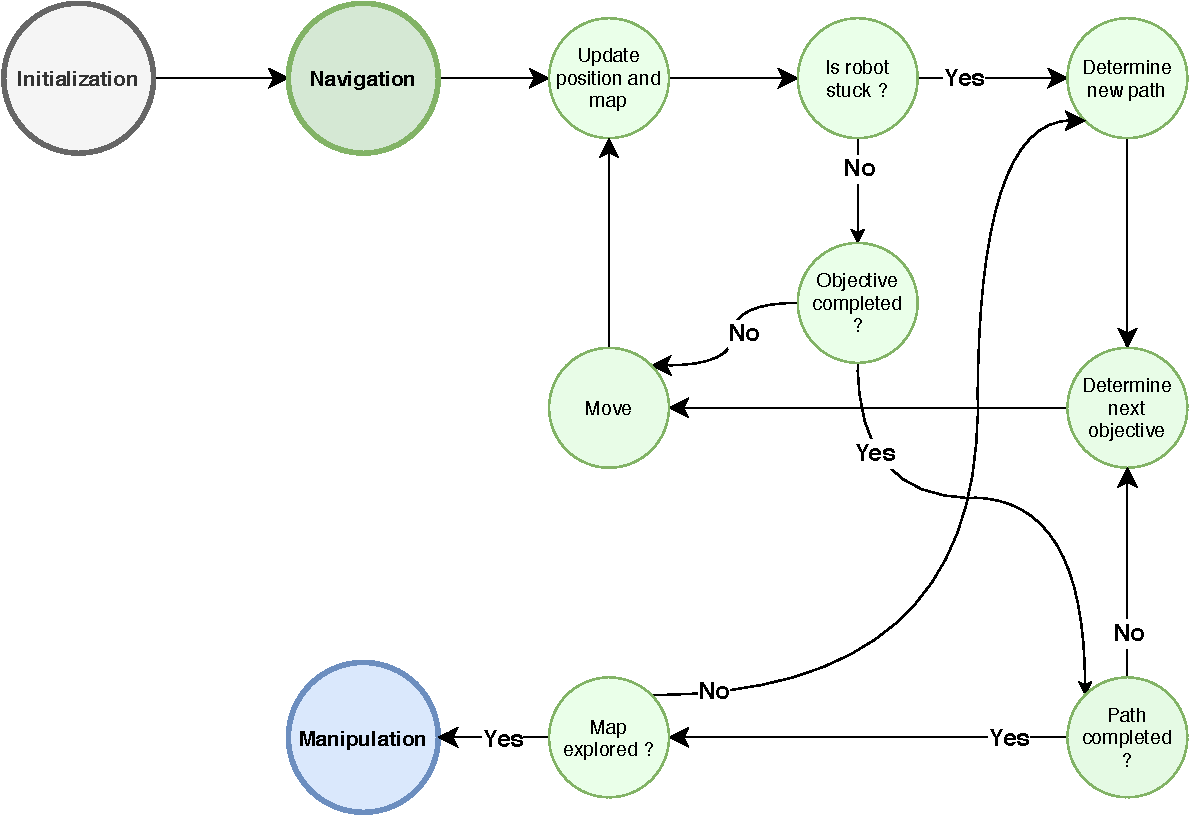
\includegraphics[width=0.8\textwidth]{resources/pdf/fsm.pdf}
        \caption{Finite state machine for the Milestone (a).}
        \label{fig:fsm}
    \end{figure}
\end{document}
